% Chapter Template

\chapter{Statistical Theory} % Main chapter title

\label{ChapterX} % Change X to a consecutive number; for referencing this chapter elsewhere, use \ref{ChapterX}

%----------------------------------------------------------------------------------------
%	SECTION 1
%----------------------------------------------------------------------------------------

\section{Theorems}

\begin{itemize}
    \item \textbf{Bayes Theorem:}
    First, let's define a partition:
    The events $C_1, C_2, \dots, C_k$ form a partition of the sample space $\Omega$, if $\Omega = \bigcup^k_{i=1}C_i$ and $C_i \bigcap C_j = \varnothing, \forall_{i \neq j}$
    
    Second, let's define the Law of Total Probability:
    If $C_1, C_2, \dots, C_k$ form a partition of the sample space $\Omega$ and $A \in \digamma$, then:
    
    \begin{equation}
        P(A) = \sum^{k}_{i=1}P(A \cap C_i) = \sum^{k}_{i=1}P(A|C_i)P(C_i)
    \end{equation}
    
    Finally, the Bayes Theorem:
    If $C_1, C_2, \dots, C_k$ form a partition of the sample space $\Omega$ and $A \in \digamma$, then:
    \begin{equation}
        P(C_j|A) = \frac{P(A|C_j)P(C_j)}{\sum^{k}_{i=1}P(A|C_i)P(C_i)}, j=1, 2, \dots, k
    \end{equation}

    \item \textbf{Strong Law of the Large Numbers:}
    Let $X_1, X_2, \dots, X_n$ be a sequence of i.i.d random variables with expected value $EX_i = \mu$. Then, with probability 1, 
    
    \begin{equation}
        \frac{X_1 + X_2 + \dots + X_n}{n} \to \mu \text{ when } n \to \infty
    \end{equation}
    
    \item \textbf{The Central Limit Theorem:}
    
    Let $X_1, X_2, \dots, X_n$ be a sequence of i.i.d random variables with expected value $EX_i = \mu < \infty$ and variance $0 < Var(X_i) = \sigma^2 < \infty$. Then, the random variable
    
    \begin{equation}
        Z_n = \frac{\bar{X} - \mu}{\sigma/\sqrt{n}} = \frac{X_1 + X_2 + \dots + X_n - n\mu}{\sqrt{n}\sigma}
    \end{equation}
  
    converges in distribution to the standard normal random variable as $n$ goes to infinity, that is
    
    \begin{equation}
        \lim_{n \to +\infty} P(Z_n \leq x) = \Phi (x), for all x \in \mathbb{R}
    \end{equation}
    
    where $\Phi (x)$ is the standard normal CDF.

\end{itemize}

\section{Estimation}
\begin{itemize}
    \item \textbf{Maximum likelihood estimation:} in statistics, maximum likelihood estimation (MLE) is a method of estimating the parameters of an assumed probability distribution, given some observed data. This is achieved by maximizing a likelihood function so that, under the assumed statistical model, the observed data is most probable. The point in the parameter space that maximizes the likelihood function is called the maximum likelihood estimate.The logic of maximum likelihood is both intuitive and flexible, and as such the method has become a dominant means of statistical inference.
    
    The method of maximum likelihood is, by far, the most popular technique for deriving estimators. Recall that if $X_1, X_2, \dots, X_n$ are an i.i.d sample from a population with pdf or pmf $f(x|\theta_1, \dots, \theta_k)$, the likelihood function is defined by
    
    \begin{equation}
        L(\theta|\bold{x}) = L(\theta_1, \dots, \theta_k|x_1, \dots, x_k) = \prod^{n}_{i=1}f(x_i|\theta_1, \dots, \theta_k)
    \end{equation}
    
    Maximum-likelihood estimators have no optimum properties for finite samples, in the sense that (when evaluated on finite samples) other estimators may have greater concentration around the true parameter-value.However, like other estimation methods, maximum likelihood estimation possesses a number of attractive limiting properties: As the sample size increases to infinity, sequences of maximum likelihood estimators have these properties: 
    
    \begin{enumerate}
        \item Consistency: the sequence of MLEs converges in probability to the value being estimated ($\hat{\theta}_n \xrightarrow {p} \theta$), i.e, 
        
        \begin{equation}
            P(|\hat{\theta}_n - \theta| > \epsilon) \to 0, \text{ as } n \to \infty
        \end{equation}
        
        \item Functional equivariance;
        \item Efficiency, i.e. it achieves the Cramér–Rao lower bound when the sample size tends to infinity. This means that no consistent estimator has lower asymptotic mean squared error than the MLE (or other estimators attaining this bound), which also means that MLE has asymptotic normality.
        
        \begin{equation}
            {\sqrt {n\,}}\,\left({\widehat {\theta \,}}_{\text{mle}}-\theta_0\right)\ \ \xrightarrow {d} \ \ {\mathcal {N}}\left(0,\ {\mathcal {I}(\theta_{0})}^{-1}\right)~,
        \end{equation}
        where $\mathcal {I}$ is the Fisher Information Matrix.
        
        If asymptotic normality holds, then asymptotic efficiency falls out because it immediately implies
        
        \begin{equation}
            \hat{\theta} \ \xrightarrow {d} \ \ {\mathcal {N}}\left(\theta_0,\ (\mathcal {I}_{n}(\theta_0))^{-1}\right)~,
        \end{equation}
         
         I use the notation $\mathcal{I}_{n}$ for the Fisher Information for $X = (X_1, \dots, X_n)$ (finite sample) and $\mathcal {I}$ for the Fisher Information for a single $X_i \in X$. Therefore, if the data provided are i.i.d, $\mathcal{I}_{n} = n\mathcal {I}$
         
        \item Second-order efficiency after correction for bias.
    \end{enumerate}
    
    The asymptotic distribution of the MLE estimators can be used for constructing approximate confidence intervals. Alternatively, bootstrap confidence intervals can also be constructed and this may be especially suitable for small sample sizes.
    
    \item \textbf{Bayes estimators:} in the classical approach, the parameter, $\theta$, is thought to be an unknown, but fixed quantity.  A random sample $X_1, X_2, \dots, X_n$ is drawn from a population indexed by $\theta$ and, based on the observed values in the sample, knowledge about the value of $\theta$ is obtained. In the Bayesian approach $\theta$ is considered a quantity whose variation can be described by a probability distribution (called the \textit{prior distribution}). This is subjective distribution, based on the experimenter's belief and is formulated before the data are seen (hence the name prior distribution). A sample is then taken from a population indexed by $\theta$ and the prior distribution is updated with this samples information. The updated prior is called the \textit{posterior distribution} This updating is done with the use of Baye's Rule, hence the name Bayesian statistics.
    
    \begin{equation}
        \pi(\theta|\bold{x}) = \frac{f(\bold{x}|\theta)\pi(\theta)}{\int f(\bold{x}|\theta)\pi(\theta) d\theta}
    \end{equation}
    
    Notice that the posterior distribution is a conditional distribution, conditional upon observing the sample. The posterior distribution is now used to make statements about $\theta$, which is still considered a random quantity. For instance, the mean of the posterior distribution can be used as a point estimate to $\theta$:
    
    \begin{equation}
        \hat{\theta} = E(\theta|\bold{x})
    \end{equation}
\end{itemize}

\section{Some key concepts}

\subsection{Confidence Interval}
Importante lembrar que um intervalo de confiança é utilizado para um parâmetro e não para uma variável aleatória. Se pudéssemos construir uma quantidade grande de intervalos (aleatórios) (lim inf, lim sup) (todos baseados em amostras de tamanho n, 95\% deles conteriam o parâmetro $\mu$)

\begin{figure}[H]
\centering
\caption{ConfidenceInterval}
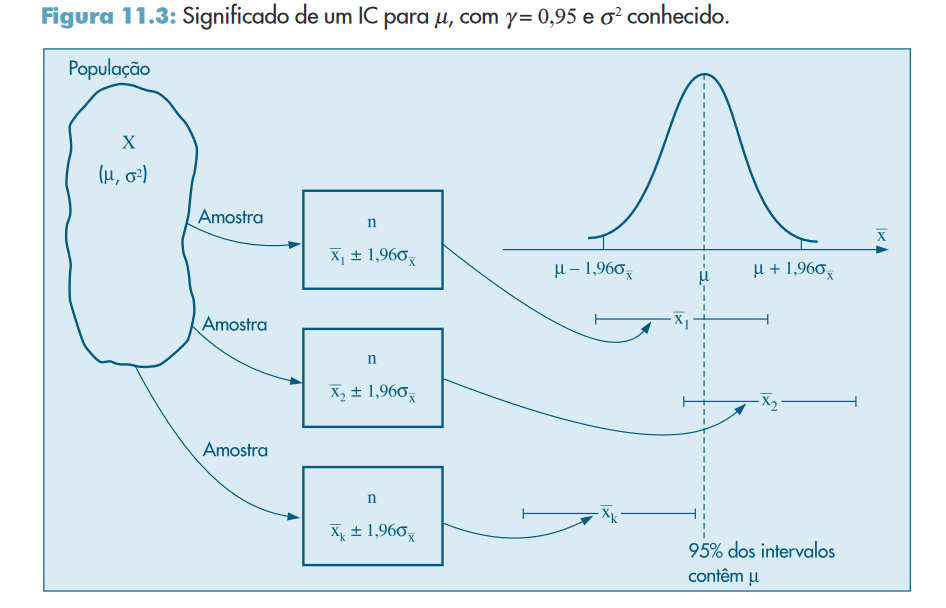
\includegraphics[scale=.5]{Figures/confidence-interval.PNG}
\end{figure}

\subsection{Bootstrapping}
Método de reamostragem que trata uma amostra como uma população finita; então são geradas amostras a partir da original, para estimar característica populacionais e fazer infêrencia sobre a população.

É uma classe de métodos de Monte Carlo não paramétricos que estimam a distribuição da população por reamostragem.

O termo “bootstrap” pode ser dirigido a bootstrap não-paramétrico ou bootstrap
paramétrico. Seguiremos com o primeiro.

A distribuição da população finita representada pela amostra pode ser encarada como uma pseudo-população, com características análogas às da verdadeira população. Através da geração repetida de amostras aleatórias, com reposição, desta pseudo-população (reamostragem), a distribuição de amostragem de uma estatística pode ser estimada. 

O bootstrap gera amostras aleatoriamente a partir da distribuição empírica da amostra.

Propriedades de um estimador tal como o viés ou o erro padrão podem ser estimadas
por reamostragem.


É possível utilizar bootstrapping para calcular um intervalo de confiança para avaliar a acurácia de um modelo em um conjunto de dados de teste. Inclusive, para estudar AUCROC.

\subsection{Methods of Evaluating Estimators}

\begin{itemize}
    \item \textbf{Standard Error (Erro Padrão)}: According to Bussab, if $\hat{\theta}$ is a estimator for $\theta$, we call the standard error (erro padrão) of $\hat{\theta}$ the following quantity:
    
    \begin{equation}
        EP(\hat{\theta}) = \sqrt{Var(\hat{\theta})}
    \end{equation}
    
    The variance of $\hat{\theta}$ depends of distribution parameters. Generally, to obtain an estimate of the standard error, we use:
    
    \begin{equation}
        \hat{EP(\hat{\theta})} = \sqrt{\hat{Var(\hat{\theta})}}
    \end{equation}
    
    The standard error for the mean $\bar{X}$ of a sample of size $n$ is $\sqrt{Var(X)/n}$
    
    \item \textbf{Mean Square Error (MSE) of an Estimator:} the mean square error (MSE) of an estimator $\hat{\theta}$ of a parameter $\theta$ is $E[(\hat{\theta} - \theta)^2]$. Do not confuse the MSE with the RMSE used to evaluate the predictions of a regression model.

\end{itemize}

\subsection{Fisher Information:} in mathematical statistics, the Fisher information (sometimes simply called information) is a way of measuring the amount of information that an observable random variable X carries about an unknown parameter $\theta$ of a distribution that models X.
    
    \begin{equation}
        \mathcal {I}(\theta )=\operatorname {E} \left[\left.\left({\frac {\partial }{\partial \theta }}\log f(X;\theta )\right)^{2}\right|\theta \right]=-\operatorname {E} \left[\left.\left({\frac {\partial^2 }{\partial \theta^2 }}\log f(X;\theta )\right)\right|\theta \right]=\int _{\mathbb {R} }\left({\frac {\partial }{\partial \theta }}\log f(x;\theta )\right)^{2}f(x;\theta )\,dx,
    \end{equation}
    
\subsection{Hessian Matrix:} Suppose $f:\mathbb{R}^n \to \mathbb{R}$ is a function taking as input a vector $\bold{x} \in \mathbb{R}^n$ and outputting a scalar $f(\bold{x}) \in \mathbb{R}$. If all second partial derivatives of $f$ exist, then the Hessian matrix $\bold{H}$ of $f$ is a square $n \times n$, usually defined and arranged as follows:
    
    \begin{equation}
        \mathbf {H} _{f}={\begin{bmatrix}{\dfrac {\partial ^{2}f}{\partial x_{1}^{2}}}&{\dfrac {\partial ^{2}f}{\partial x_{1}\,\partial x_{2}}}&\cdots &{\dfrac {\partial ^{2}f}{\partial x_{1}\,\partial x_{n}}}\\[2.2ex]{\dfrac {\partial ^{2}f}{\partial x_{2}\,\partial x_{1}}}&{\dfrac {\partial ^{2}f}{\partial x_{2}^{2}}}&\cdots &{\dfrac {\partial ^{2}f}{\partial x_{2}\,\partial x_{n}}}\\[2.2ex]\vdots &\vdots &\ddots &\vdots \\[2.2ex]{\dfrac {\partial ^{2}f}{\partial x_{n}\,\partial x_{1}}}&{\dfrac {\partial ^{2}f}{\partial x_{n}\,\partial x_{2}}}&\cdots &{\dfrac {\partial ^{2}f}{\partial x_{n}^{2}}}\end{bmatrix}}
    \end{equation}
\end{itemize}